\documentclass[conference]{IEEEtran}
\IEEEoverridecommandlockouts
% The preceding line is only needed to identify funding in the first footnote. If that is unneeded, please comment it out.
\usepackage{cite}
\usepackage{amsmath,amssymb,amsfonts}
\usepackage{algorithmic}
\usepackage{graphicx}
\usepackage{textcomp}
\usepackage{xcolor}
\usepackage{hyperref}
\usepackage{graphicx}
\usepackage{smartdiagram}

\def\BibTeX{{\rm B\kern-.05em{\sc i\kern-.025em b}\kern-.08em
    T\kern-.1667em\lower.7ex\hbox{E}\kern-.125emX}}
\begin{document}

\title{A Wikipedia Tour of Death - Or How University College Boat Club Became Popular\\
{\footnotesize Network Tour of Data Science Report, January 2019}
}

\author{Isabela Constantin, Ad\'elie Garin, Celia Hacker, Michael Spieler}

\maketitle

\section{Introduction}
Using the Wikipedia data set that is now open source, we would like to understand how the number of views on one page spreads in the linked pages when some unexpected event happens. We chose to study specifically the pages of three famous people who died in the past few years and we are interested in the number of views in the pages that are related to the main page of the person who died. We will consider two times for the number of views: the day before the person dies and the day of the death. 

\medskip

For each person who died, we build a specific graph around their wikipedia page by taking wikipedia pages as nodes and links from one page to another as directed edges. We will use both the directed graph, in which one page which is linked to the other leads to only one direction for the concerned edge, and the undirected graph, for which there exists an edge if and only if there is one page linked to the other. The full construction of the three graphs is described in Section \ref{acquisition}. For each node $i$ (corresponding to a wikipedia page) of a graph, we are interested in the following quotient: \[Q_i:=\frac{\text{number of views of the page on the day of death }}{\text{number of views of the page the day before}}.\] The higher this value is, the bigger difference there is between the number of views of the node $i$ on the day before the person died and the day of their death. 

\medskip

The question we ask ourselves is the following: does the number of views on the pages related to the one of the famous person depend on the number of views of the page of the person itself? 

\medskip

To answer this question, we will study the quotient $Q_i$ for each node $i$ of the graph and analyse the different values $Q_i$  as a signal on the graph. We build a general pipeline to analyse the three graphs in the same matter, to be able to compare them. Our general pipeline is the following: 

\begin{center}
\smartdiagramset{border color=none,
set color list={blue!50!cyan,green!60!lime,orange!50!red,red!80!black},
back arrow disabled=true}

\smartdiagram[flow diagram:horizontal]{Data Acquisition,Data Exploration,Data Exploitation}
\end{center}

We first start by acquiring the data and building the three graphs around the people we chose, in Section \ref{acquisition}. Then, we explore the graphs and try to extract their general properties in Section \ref{exploration}. In Section \ref{exploitation}, we exploit the data, trying to test our hypothesis and we finally draw conclusions in Section \ref{conclusion}. All the code used for this report is available in \cite{Repo}. 

\section{Data Acquisition} \label{acquisition}

We constructed the graphs around the selected Wikipedia articles corresponding to each of the following people: Stephen Hawking \cite{stephenhawking}, Stan Lee \cite{stanlee} and Alan Rickman \cite{alanrickman}. To make it easier for the following description, we will say that a node or page \textit{links in} another one if there is a link from the former to the latter, and \textit{links out} if the link is from the latter to the former. We grew the graphs around the main pages (Stephen Hawking, Stan Lee, Alan Rickman) by selecting the pages linked out from the main ones (step $1$), then we added pages linked out from the pages at step $1$ (step $2$), and so on. At each step $i$, we hence added pages that were linked out from the previous pages of step $i-1$. Essentially, we crawled the pages by a slightly modified version of Bread First Search. 

\subsection{Sampling}
It would be too much data to add all the linked out pages at each step.  To reduce the amount of data, we  subsampled by making several choices of parameters, described as follow. First, we randomly subsampled the nodes by giving a higher probability of being added in the graph to the pages which link is higher (in order of appearance) in previous pages. This is because pages that are stated early in a Wikipedia page are more likely to be really related to the subject of the page. We hence set up two percentage parameters $\theta_1$ and $\theta_2$. Let us take a page at step $i$. The first $\theta_1$ percent of links from that page constitute for $\theta_2$ percent of the edges linked out from this page at step $i+1$. Our next choice of parameter is the number of neighbors for the main page, i.e. the number of pages that will be taken at step $1$. We call this parameter $N_{step1}$. We also assign a minimum of popularity parameter, $m_{pop}$, which is the minimum number of out-links on a page for the page to be considered as a possible node. The last parameter that we can set up is the maximal number of nodes $N_{max}$. 

\medskip 

The parameters are summed up in the following table. 

\begin{table}[htbp]
\caption{Parameters}
\begin{center}
\begin{tabular}{|c|c|c|c|}
\hline
 & Use & Name in code & Value \\
\hline
$\theta_1$& Top  percentage of links  & percentage$\_1$ & 0.2 \\
\hline
$\theta_2$& Percentage of subsampled links &  percentage$\_1\_$subsample &  0.5\\
\hline
$N_{step1}$  &  Number of pages taken at step 1   & n$\_$links$\_$hop1  & 150  \\
\hline
$m_{pop}$  & Mimimum popularity  & min$\_$popularity &30 \\
\hline
$N_{max}$  &  Max number of nodes & max$\_$nodes&  2701 \\
\hline
\end{tabular}
\end{center}
\end{table}

We set up the values of the parameters for the pages that are important and related to the subject to have a higher probability to be in the graphs. We chose them such that the top $20$ percent of the links account for $50$ percent of the sampled links (parameters $\theta_1$ and $\theta_2$). At step $1$, we added $150$ links (parameter $N_{step1}$). To be considered as a possible node, a page needed at least $30$ out-links (parameter $m_{pop}$). Last but not least, the maximum number of nodes in the graph, $N_{max}=2701$, was selected at random between $150 \times 3 \times 3$ and $150 \times 3 \times 3 \times 3$ to make sure that we would have at least $5$ steps in the process. Indeed, at each step we added on average $3$ links from each node, and we started with $150$ nodes after step $1$.


\medskip

The resulting graphs are directed, unweighted and connected. 

\subsection{Building the views signal}
We found the number of views and extracted them at each page for the day before the death of the person and the day of the death. 
For each page $i$  we computed the quotient  \[Q_i:=\frac{\text{number of views of the page on the day of death }}{\text{number of views of the page the day before}},\] and we assign this value to the corresponding node of the graph. Taking this quotient is a sort of normalization of the number of views. The higher this value is, the more the number of views on the day of the death is big compared to the number of views of the day before.  In Section \ref{exploitation}, we consider these values as a signal on the graph and we study their diffusion. 

\section{Data Exploration} \label{exploration}

In this section, we analyse basic properties of the graphs.  One point can be made with this section: an analysis of the same signal on those three graphs would make sense, because the three graphs are very similar. 

\medskip

Let us first summarize the number of views of the pages for Stephen Hawking, Stan Lee and Alan Rickman. 

\begin{table}[htbp]
\caption{Number of views}
\begin{center}
\begin{tabular}{|c|c|c|c|}
\hline
 Views & Day of death &Day before & Quotient \\
\hline
\textbf{Stephen Hawking} & 7126234 & 15781 &  451.57 \\
\hline
 \textbf{Stan Lee} &2404717 & 6929 &  347.05 \\
\hline
\textbf{Alan Rickman} & 3394010 & 3664 & 926.31 \\
\hline
\end{tabular}
\end{center}
\end{table}

We can clearly see that the number of views grew a lot on the day of the death of each of them. The quotients are of the same order.

\medskip

We also computed the graphs of the number of views several days before and after the death just for those three pages. 

\begin{figure}[!htb] \label{views}
\minipage{0.15\textwidth}
  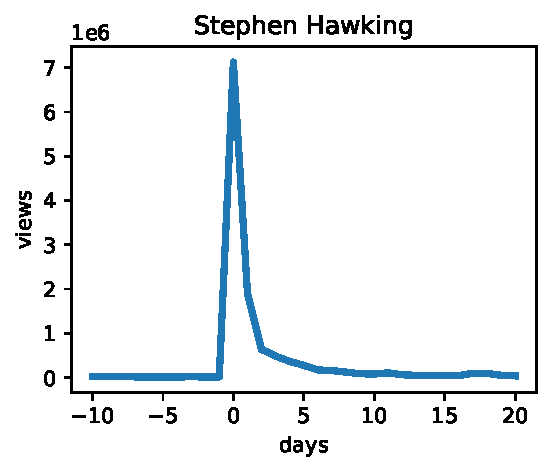
\includegraphics[width=\linewidth]{viewsSH.pdf}
\endminipage\hfill
\minipage{0.15\textwidth}
  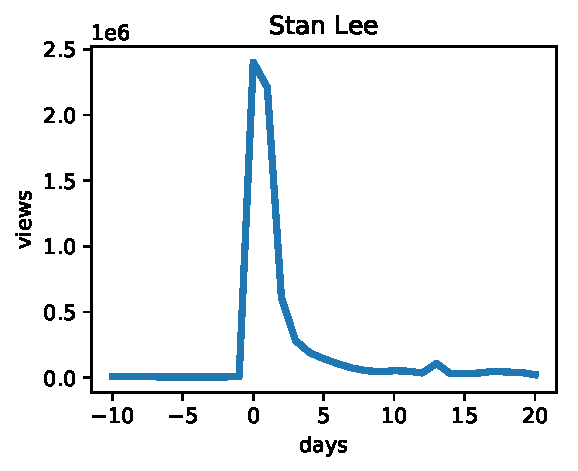
\includegraphics[width=\linewidth]{viewsSL.pdf}
\endminipage\hfill
\minipage{0.15\textwidth}%
  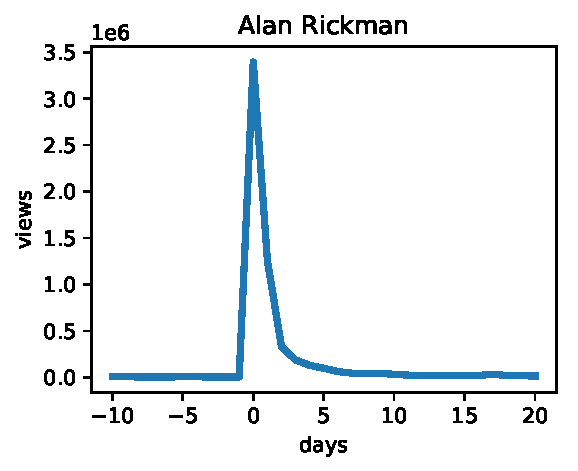
\includegraphics[width=\linewidth]{viewsAR.pdf}
\endminipage
\caption{Number of views for Stephen Hawking, Stan Lee and Alan Rickman. For each person, we can see that there is a high peak of views on the days of the death, then the number of views quickly decays to the baseline.  }
\end{figure}

\subsection{Basic properties}
We start by analysing some basic properties of each graph, such as the number of nodes, the number of edges, the diameter of the (undirected) graph, and the average clustering coefficient (ACC), number of triangles and global clustering coefficient (GCC) with the tools available in Networkx. The results are stated in the  following table. 


\begin{table}[htbp]
\caption{Basic properties of the graphs}
\begin{center}
\begin{tabular}{|c|c|c|c|}
\hline
 Properties & \textbf{Stephen Hawking}& \textbf{Stan Lee}& \textbf{Alan Rickman} \\
\hline
$\#$nodes& 2701 &  2701 & 2701 \\
\hline
$\#$edges & 26921 & 33469 & 28012  \\
\hline
Diameter & 7 & 7 &  8\\
\hline
ACC & 0.138 & 0.131 &  0.123\\
\hline
$\#$triangles  & 41973 & 60096 & 38076  \\
\hline
GCC & 0.000335 & 0.000379 & 0.000251 \\
\hline
\end{tabular}
\end{center}
\end{table}

The number of nodes are the same because they were set to be the same. The number of edges are of the same order, as well as the diameters and average and global clustering coefficients. This comes partially from the way the graphs were built in the same way and partially from the fact that we built them around very similar type of pages, famous people. The number of triangles is slightly higher for Stan Lee, most likely because there are more edges in the graph. Both the average clustering coefficient and the global clustering coefficient are very low. This comes from the construction of the graphs, they were built around one node, adding edges one by one. Hence, very few triangles are built on the way. 

\subsection{Adjancency matrices}
 The following figure shows the adjacency matrices of the undirected graphs.
 
\begin{figure}[!htb]
  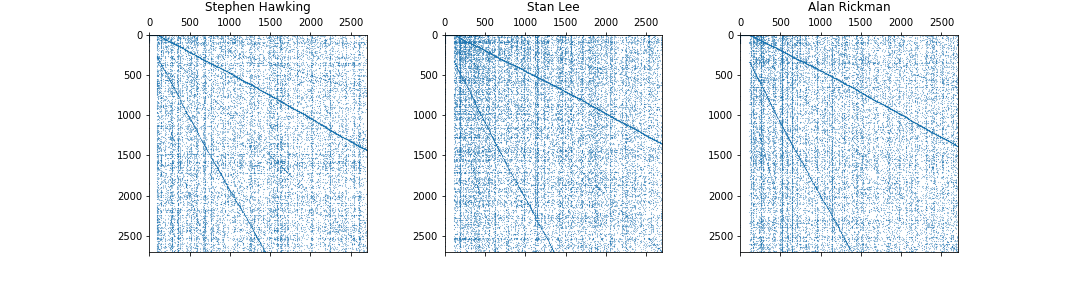
\includegraphics[width=\linewidth]{matrices.png}
\caption{Undirected ajacency matrices for Stephen Hawking, Stan Lee and Alan Rickman's graphs. }
\end{figure}

The three matrices are very similar. The straight lines "in diagonal" that appear in the three of them come from the construction of the graphs. The graphs were built by "chains", we start with one node and add many edges out of it. This will create a lot of entries nearby in the adjancency matrix. Starting from node $i$, a node $j$ is added, linked out to $i$. Then a node $k$ is added, linked out to $j$, and so on, with $i$, $j$, and $k$ quite close to each other. This gives those lines structure in the matrices. 

\subsection{Degree Distribution}

Here we study the degree distributions of each graph. We computed degree distributions with logarithmic scale for in-degrees, out-degrees and undirected case. 

\begin{figure}[!htb]

\minipage{0.15\textwidth}
  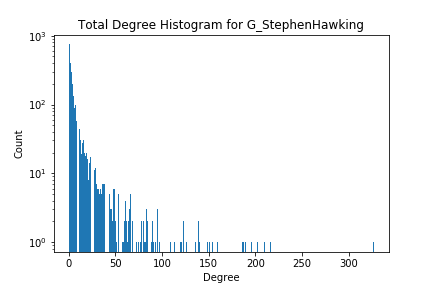
\includegraphics[width=\linewidth]{degreeSH.png}
\endminipage\hfill
\minipage{0.15\textwidth}
  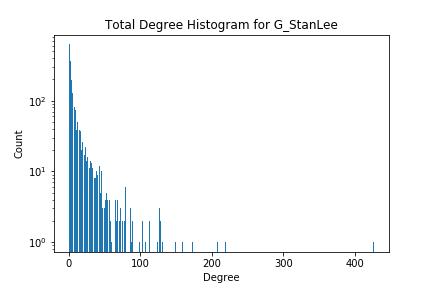
\includegraphics[width=\linewidth]{degreeSL.png}
\endminipage\hfill
\minipage{0.15\textwidth}%
  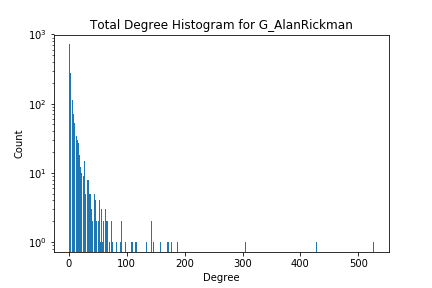
\includegraphics[width=\linewidth]{degreeAR.png}
\endminipage

\minipage{0.15\textwidth}
  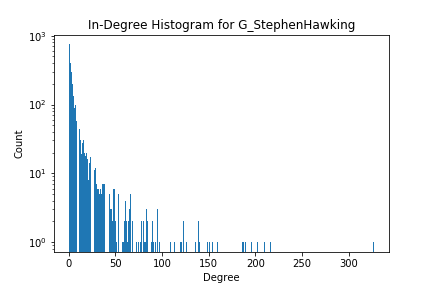
\includegraphics[width=\linewidth]{degreeinSH.png}
\endminipage\hfill
\minipage{0.15\textwidth}
  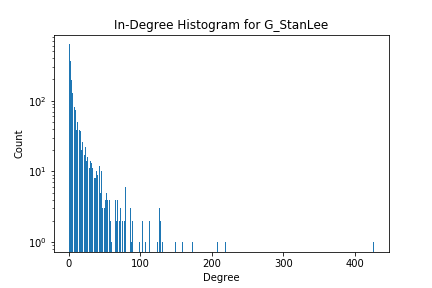
\includegraphics[width=\linewidth]{degreeinSL.png}
\endminipage\hfill
\minipage{0.15\textwidth}%
  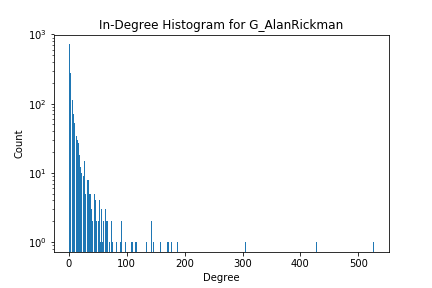
\includegraphics[width=\linewidth]{degreeinAR.png}
\endminipage

\minipage{0.15\textwidth}
  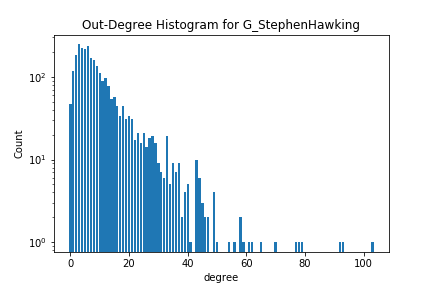
\includegraphics[width=\linewidth]{degreeoutSH.png}
\endminipage\hfill
\minipage{0.15\textwidth}
  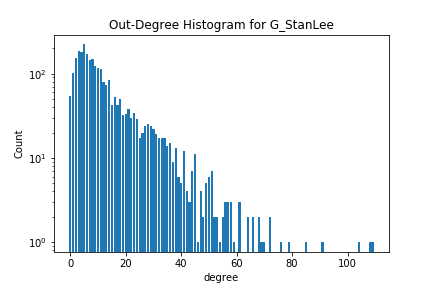
\includegraphics[width=\linewidth]{degreeoutSL.png}
\endminipage\hfill
\minipage{0.15\textwidth}%
  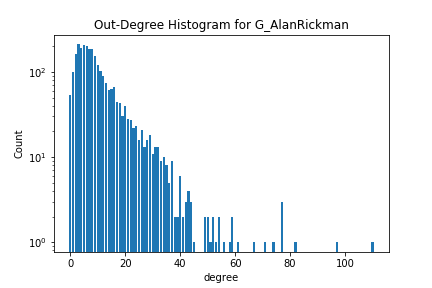
\includegraphics[width=\linewidth]{degreeoutAR.png}
\endminipage

\caption{Degree distribution of the graphs for Stephen Hawking, Stan Lee and Alan Rickman in logarithmic scale for the undirected case (top line), in-degree (middle line) and out-degree (bottom line).  }
\end{figure}

First, one can notice that the three types of degree distribution are very similar for the three graphs. There are many nodes with small degrees (in, out and total). Those are the nodes that were built at the end of the construction of the graphs. For in, out and total degrees, we can see that there are a few nodes with much higher degree. We extracted the highest degree node for each, and the results are not surprising. For out degree, Stan Lee and Alan Rickman get the highest degree for their respective graph. For the graph of Stephen Hawking, the title goes to the page "Culture of the United Kingdom", which is not that surprising as there is a section about sciences and technology that links out to many other related pages. For the in and total degrees, the three pages that get the highest degree in each graph are "United States" for Alan Rickman and Stan Lee, and "United Kingdom" for Stephen Hawking. This is not very surprising either, as those pages are cited a lot in the whole wikipedia, and our graphs do not make exceptions. In general, nodes with very high degrees are either important pages in wikipedia or very related to the people we consider. 

\subsection{Strongly Connected Components}

A directed graph is said to be strongly connected if there is a directed path connecting any two of its vertices. Our graphs are clearly connected in the undirected sense by the way we have constructed them. All of them are not strongly connected, so we computed the number of strongly connected components. Stephen Hawking's graph has $51$ strongly connected components, both Stan Lee and Alan Rickman's graphs have $55$ strongly connected components. Those numbers are relatively high. From the construction of the graphs, there are not many paths from any vertex to another one. Indeed, it is easy to go from Stan Lee to New York, for example, but more complicated to go from New York to Stan Lee. 

\section{Data Exploitation} \label{exploitation}
Note that we saw in the last Section that the graphs have very similar properties. 
We now come to the most important part of our analysis, which is the following: we consider the number of views as a signal on the graph. We would like to see how it behaves. In order to make a sensible comparison of number of views and how these number of views evolve for each graph we use the quotient of the number of views before and at the day of the event. 

\medskip
At the time of the event, pages views spike, as shown in Figure \ref{views}. Our assumption is that people visiting a page likely follow links to other pages to read more about a topic. The following figure shows the signal on the graphs and support this assumption. 

\begin{figure}[!htb] \label{circle}
  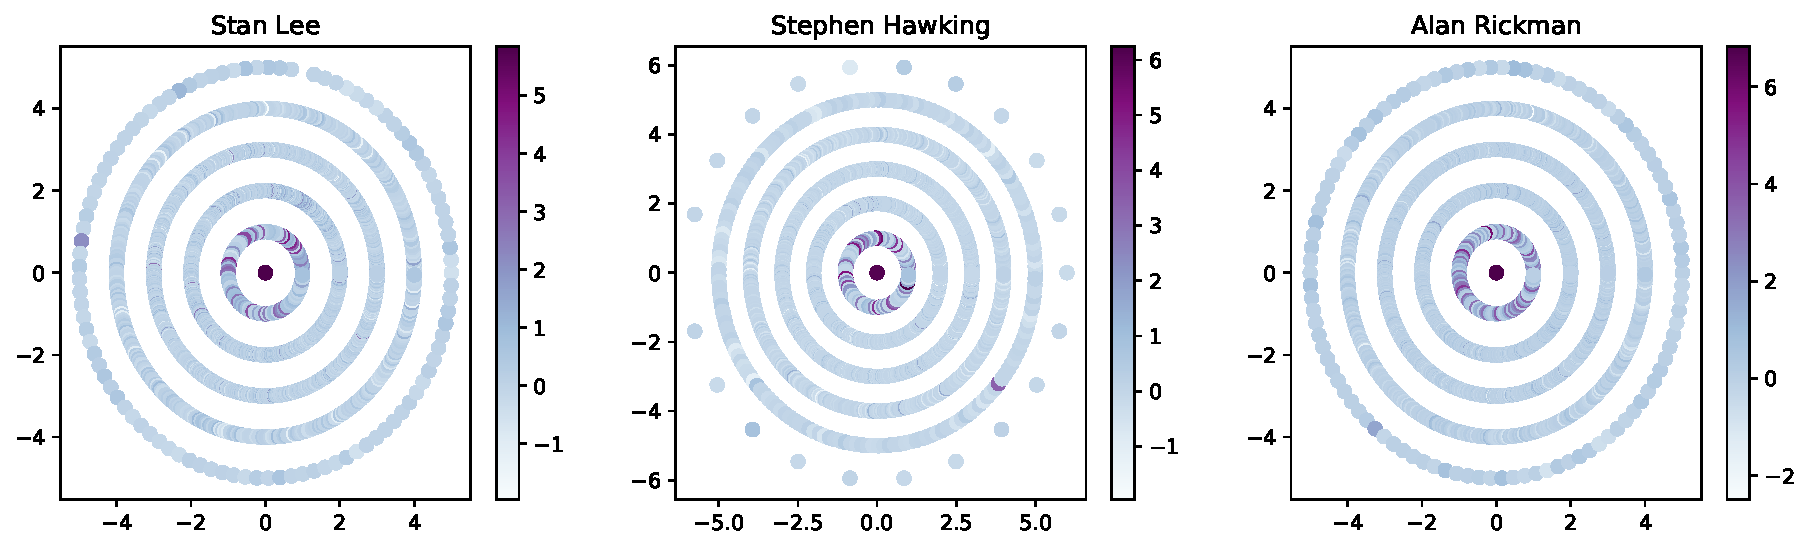
\includegraphics[width=\linewidth]{signal_scatter.pdf}
\caption{Only the nodes of the graphs are represented here. The central node of each graph stands for Stephen Hawking, Stan Lee and Alan Rickman respectively. One can see very clearly that the quotient signal is much higher in the center, near the main person, and that it decreases very fast when going away from the center.}
\end{figure}

Note that we tried several ways to represent our graph, including spectral clustering and eigenmaps, as described in \cite{clustering} and \cite{laplacian}. However, since our graphs were constructed in very specific ways, the representation in circle of Figure \ref{circle} is the best for our purpose. 

\subsection{Highest signals}
 For each page, the number of views of the day before multiplied by the signal is the number of views of the day of the death. For example, "Stan Lee" had 347.5 times more views on the day of his death than the day before. 
 
 \medskip
 
We looked at the five highest signals for each graphs. For Stephen Hawking, the nodes with highest signals are: "University College Boat Club (Oxford)"(516.00), 
"Stephen Hawking" (451.57), "Lucasian Professor of Mathematics" (268.66), "St Albans School, Hertfordshire" (180.43 ),"Keep Talking" (153.22) and "God Created the Integers" (116.60).
\newline
For Stan Lee, the nodes with highest signal are:  "Stan Lee" (347.5), "List of comics creators appearing in comics" (106.9), "Bullpen Bulletins" (82.43), "Bill Everett" (76.97), "Don Heck" (58.83 ) and "Martin Goodman (publisher)" (42.63). 
\newline
For Alan Rickman, the nodes with highest signals are: "Alan Rickman" (926.31), "Truly, Madly, Deeply" (382.86), "My Name Is Rachel Corrie" (154.50, "Tom Burke (actor)" (123.02), "Eye in the Sky (2015 film)"( 66.47) and "Adam Leonard (singer-songwriter)" (52.00). 

\medskip
Those pages have very few views in general. The reason why the signal is so high is because the number of views increased drastically thanks to the death of Stephen Hawking, Stan Lee and Alan Rickman respectively. As an example, here is the number of views of the page "University College Boat Club (Oxford)". 

\begin{figure}[!htb]
  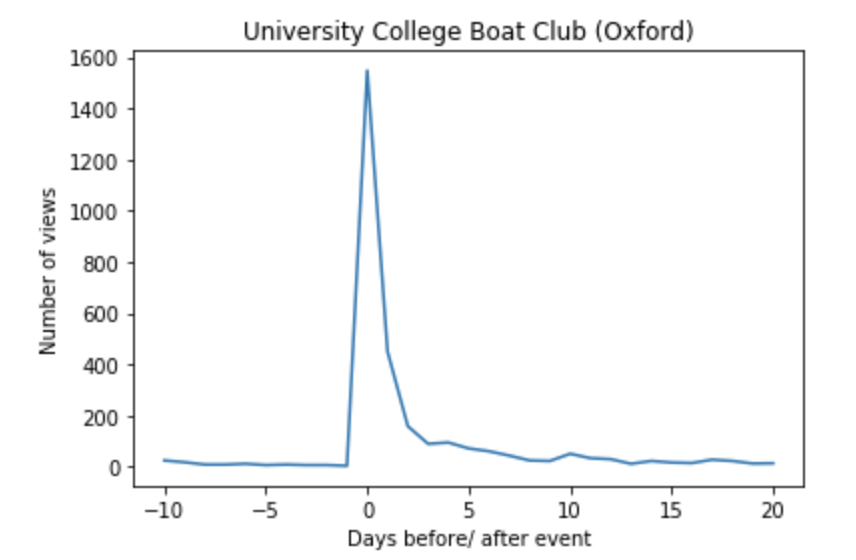
\includegraphics[width=\linewidth]{uniboat.png}
\caption{Number of views before and after the death of Stephen Hawking for the page "University College Boat Club (Oxford)". This page had almost no views before the death of Stephen Hawking, a sudden interest on the day of his death and again no interest afterwards.}
\end{figure}

\subsection{Comparison with other types of signals}

We tried to see if we can model this behaviour by applying a Dirac signal on the central node using Graph Signal Processing as introduced in \cite{signalprocessing}.
Our assumption is that our signal acts like a Dirac impulse on the main page and then spreads to the neighbouring pages. We tried to compare it to several kernels coming from a Dirac impulse. The following figure shows a Dirac impulse with a heat kernel and an inverse kernel. 

\begin{figure}[!htb]
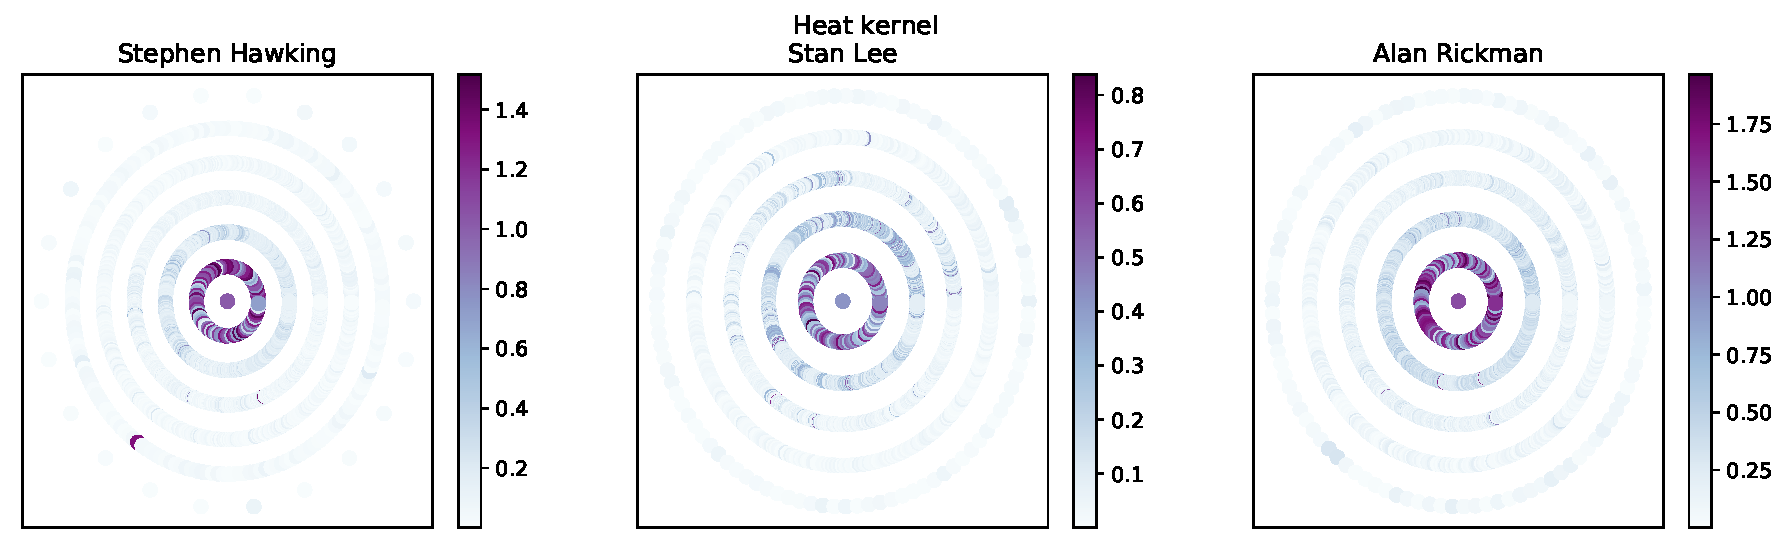
\includegraphics[width=\linewidth]{heat_scatter.pdf}
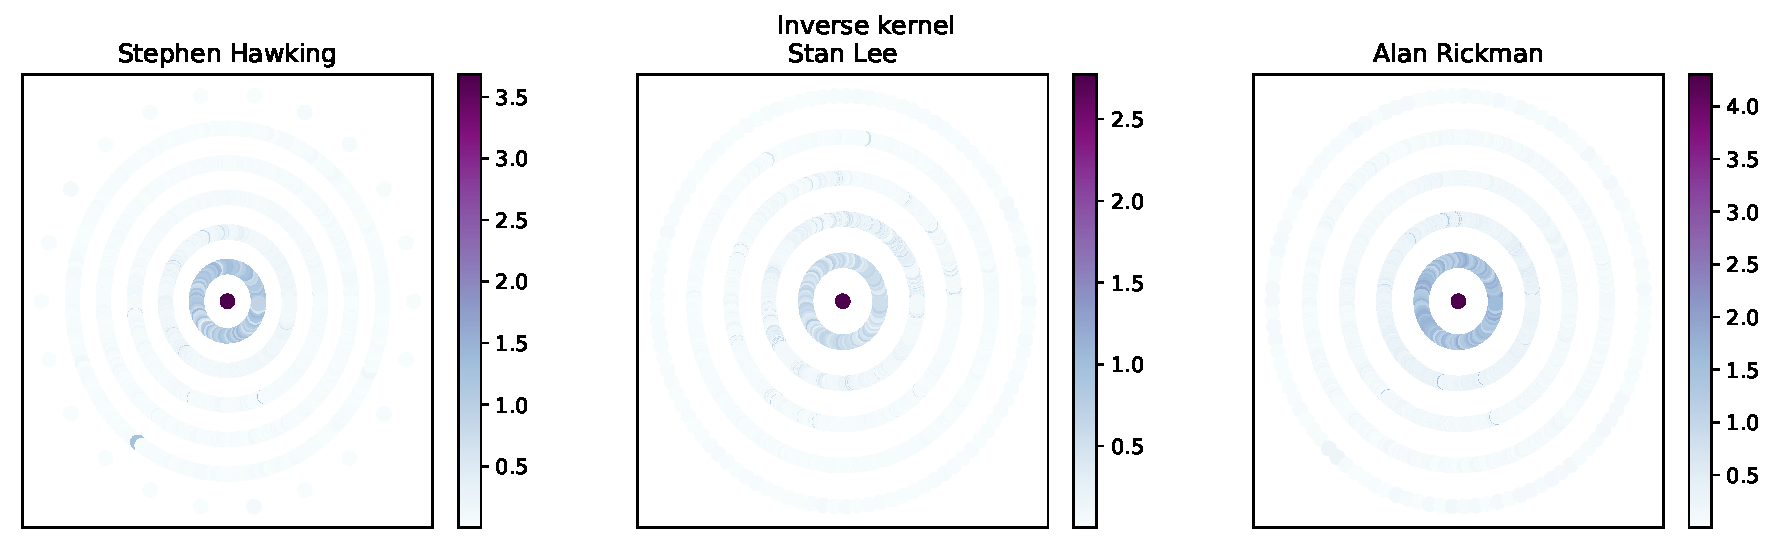
\includegraphics[width=\linewidth]{inverse_scatter.pdf}
\caption{A Dirac impulse with heat kernel (top) and inverse kernel (bottom).} 
\end{figure}

They do not look as similar to our signal as we expected. We can visually tell that the increase in views is more homogenous for the heat and inverse kernels. However, the choice of the filter time constant is not trivial. 

\medskip

We tried to find an optimal parameter to best fit the sampled signal using $L1$ and $L2$ error functions. The results are not very good, as shown on the following figure. 

\begin{figure}[!htb]
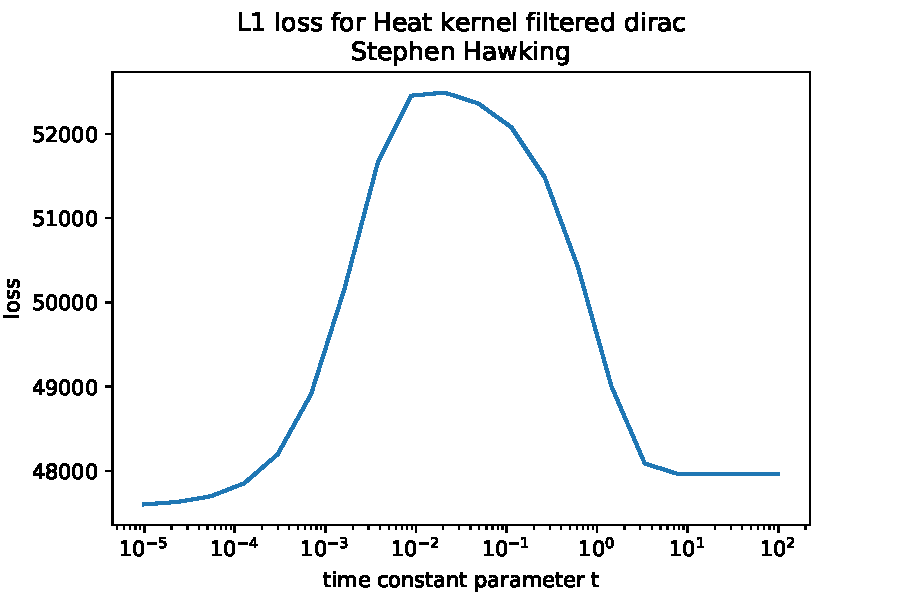
\includegraphics[width=\linewidth]{heat_loss.pdf}
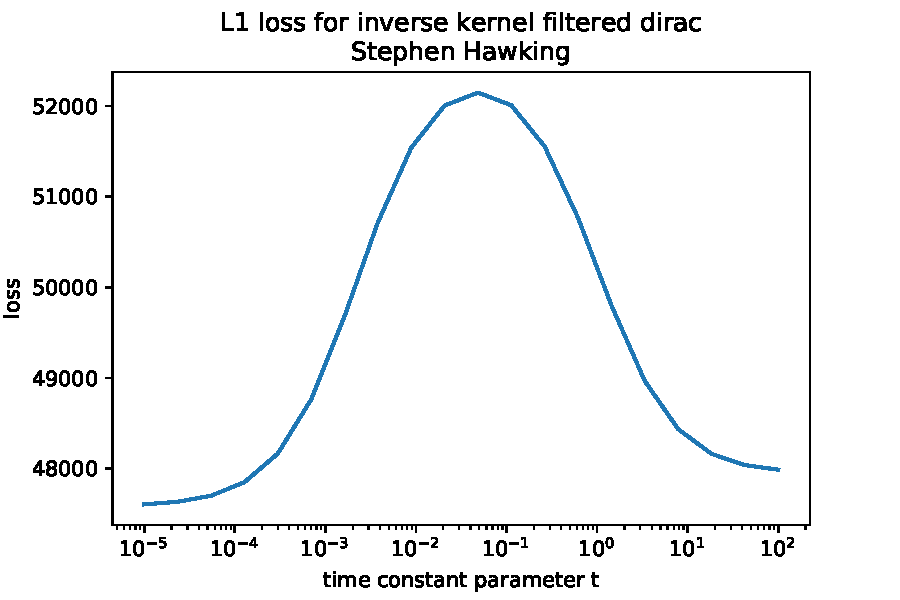
\includegraphics[width=\linewidth]{inverse_loss.pdf}
\caption{Here is the value of the error in function of the the parameter $t$ in heat (top) and inverse (bottom) kernels for the Stephen Hawking graph. The plot look similar for Stan Lee and Alan Rickman. } 
\end{figure}

We notice the error is low for extremely high and extremely low t, meaning that
the dirac input and a constant both better approximate the signal than with a heat or inverse kernel filter.

\medskip

As there does not seem to be a good parameter $t$ to fit our signal, we conclude that the filtered dirac signal is not a suitable approximation of the actual signal. Our explanation for the heat kernel is that it simulates the diffusion of a heat quantity (energy) on the graph. However, the page views is not a heat quantity that gets dispersed over the graph, it acts more like a source. Every visitor goes through the root page, which also counts as a view.

\section{Conclusion} \label{conclusion}

We tried to compare our signal to several models, and none of them fit very well in terms of loss function. The best model we could find visually is the heat kernel with parameter $t=0.1$, as shown on the following scatter plot. 

\begin{figure}[!htb]
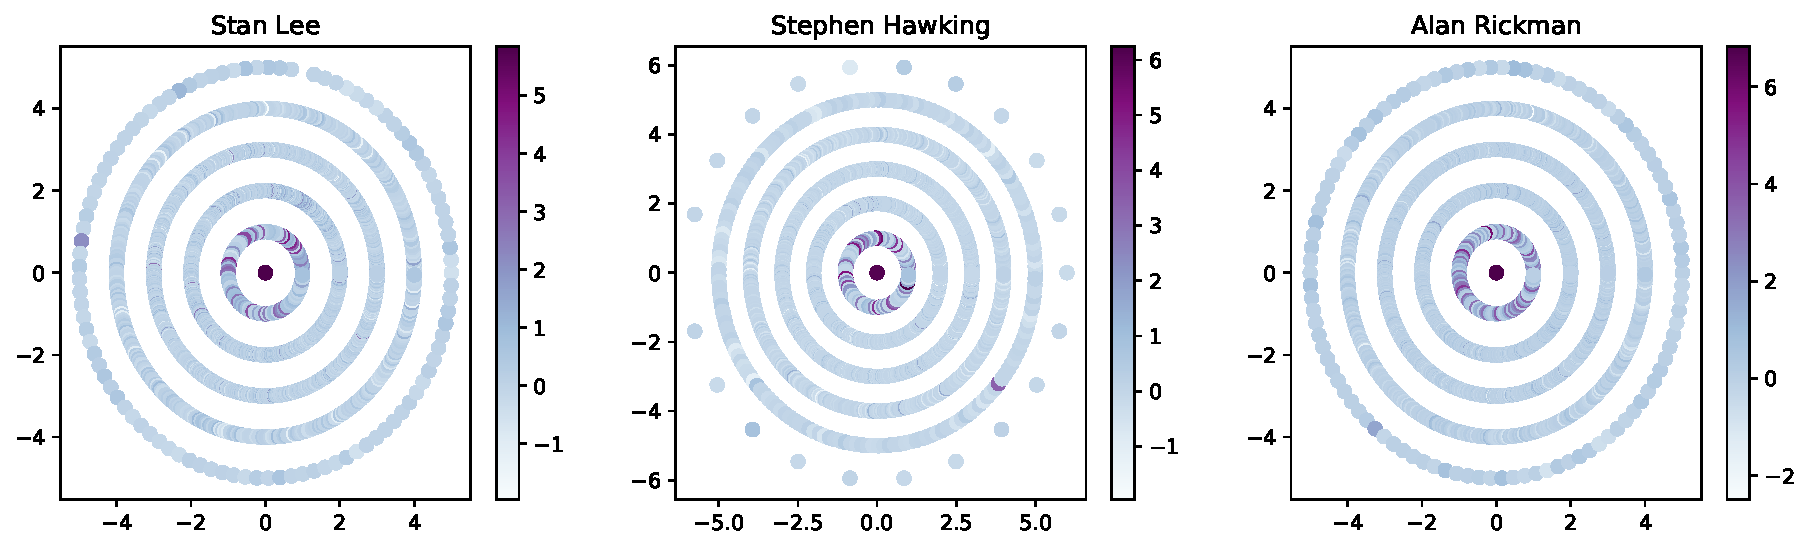
\includegraphics[width=\linewidth]{signal_scatter.pdf}
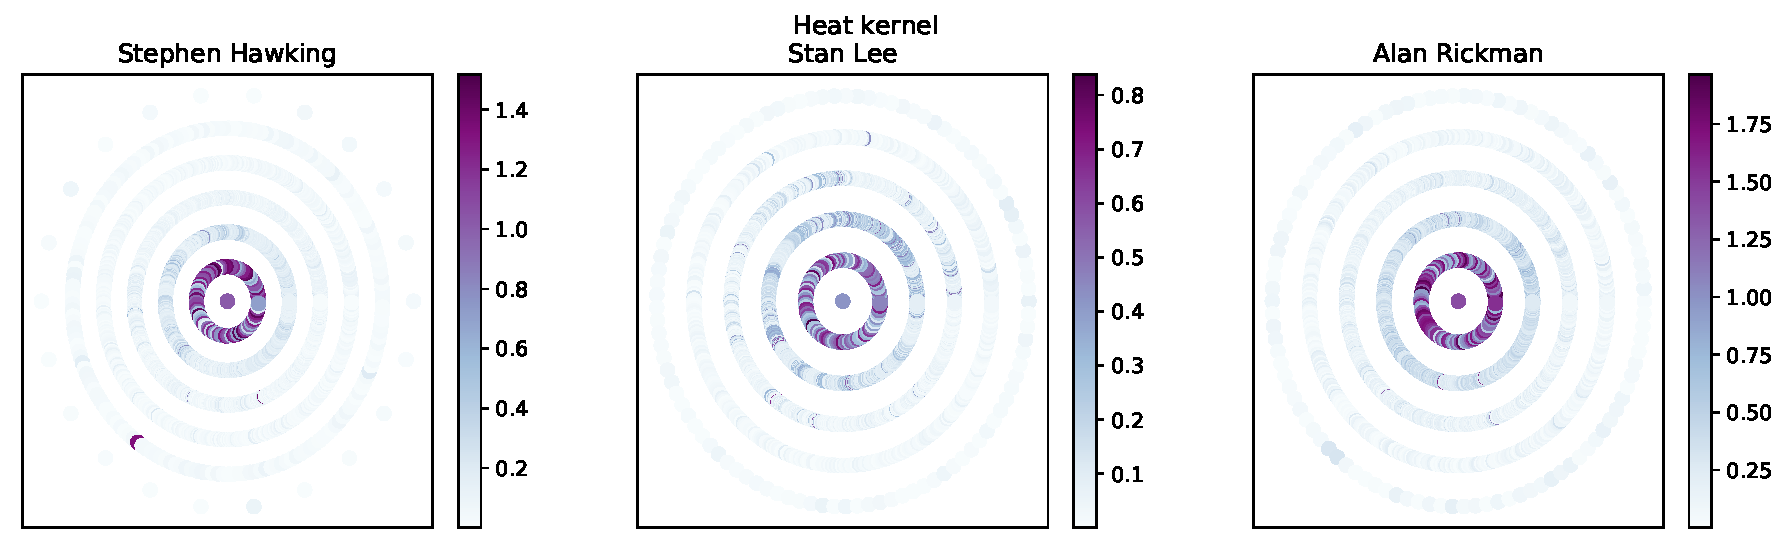
\includegraphics[width=\linewidth]{heat_scatter.pdf}
\caption{Our signal (top) and a Dirac impulse with heat kernel  with $t=0.1$ as parameter (bottom).} 
\end{figure}

Our explanation for the general behavior or the signal is the following: 
\newline
The day a famous person dies, people will visit their Wikipedia page and click on a bunch of links from there. Some of these links are barely visited usually, and hence will get a very high number of views compared to usually. If we take a page with a lot of views every day, like "United States" for example, the death of someone will not affect the number of views much. The following plot illustrates this fact. 

\begin{figure}[!htb]
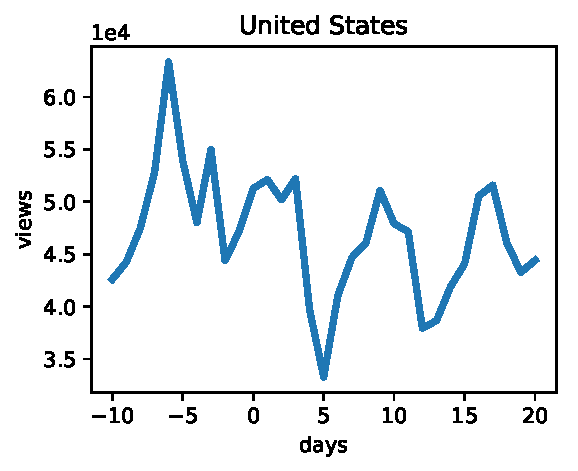
\includegraphics[width=\linewidth]{UnitedStates.pdf}
\caption{Number of views for "United States" before and after the death of Stan Lee. Clearly, the death of Stan Lee did not affect the views for this page at all.} 
\end{figure}

Note that if we had the computational power to build a graph with all the pages involved by all the events that we considered together, it would have been much more interesting to see how the number of views evolves locally on the graph. By doing the methods presented in this report, we can only do a “zoom-in” on a specific part of this big graph and analyse it independently of the rest. 

\medskip

Our final conclusion is: if you die, people will show interest in you on the day of your death, but this interest will decrease very fast. Hence, you would better not die. 


\bibliography{biblio}
\bibliographystyle{plain}

\end{document}
